%%%%%%%%%%%%%%%%%%%%%%%%%%%%%%%%%%%%%%%%%
% APA Assignment Article
% LaTeX Template
% Version 2.0 (February 7, 2023)
%
% This template originates from:
% https://www.LaTeXTemplates.com
%
% Author:
% Vel (vel@latextemplates.com)
%
% License:
% CC BY-NC-SA 4.0 (https://creativecommons.org/licenses/by-nc-sa/4.0/)
%
% NOTE: The bibliography needs to be compiled using the biber engine.
%
%%%%%%%%%%%%%%%%%%%%%%%%%%%%%%%%%%%%%%%%%

%----------------------------------------------------------------------------------------
%	PACKAGES AND OTHER DOCUMENT CONFIGURATIONS
%----------------------------------------------------------------------------------------

\documentclass[
	letterpaper, % Paper size, use either a4paper or letterpaper
	10pt, % Default font size, can also use 11pt or 12pt, although this is not recommended
	unnumberedsections, % Comment to enable section numbering
	twoside, % Two side traditional mode where headers and footers change between odd and even pages, comment this option to make them fixed
]{APAAssignment}

\addbibresource{bibliography.bib} % BibLaTeX bibliography file

\runninghead{MICS CYBER 252, Fall-2024 Hands On Lab Unit 5} % A shortened article title to appear in the running head, leave this command empty for no running head

\footertext{\textit{Hands On Lab Unit 5} (MICS CYBER 252, Fall -2024)} % Text to appear in the footer, leave this command empty for no footer text

\setcounter{page}{1} % The page number of the first page, set this to a higher number if the article is to be part of an issue or larger work

%----------------------------------------------------------------------------------------
%	TITLE SECTION
%----------------------------------------------------------------------------------------

\usepackage[title,toc,titletoc]{appendix}
\usepackage{titlesec}
\usepackage{lscape}
\usepackage{fontawesome}

\title{Hands On Lab Unit 5 \\ MICS-252, Fall 2024} % Article title, use manual lines breaks (\\) to beautify the layout

% Authors are listed in a comma-separated list with superscript numbers indicating affiliations
% \thanks{} is used for any text that should be placed in a footnote on the first page, such as the corresponding author's email, journal acceptance dates, a copyright/license notice, keywords, etc
% Affiliations are output in the \date{} command
\date{UC Berkleley School of Information \\
MICS Course 252 Fall 2024 (Kristy Westphal)
}


\author{
	Prepared by: Karl-Johan Westhoff \\
	email: \href{mailto:kjwesthoff@berkeley.edu}{kjwesthoff@berkeley.edu}
}


% % Full-width abstract
% \renewcommand{\maketitlehookd}{%
% 	\begin{abstract}
% 		\noindent Lorem ipsum dolor sit amet,rta porttitor.
% 	\end{abstract}
% }

%----------------------------------------------------------------------------------------

\setcounter{tocdepth}{5}
\setcounter{secnumdepth}{5}
\usepackage[title]{appendix}

\begin{document}
\onecolumn
\maketitle % Output the title section

%----------------------------------------------------------------------------------------
%	ARTICLE CONTENTS
%----------------------------------------------------------------------------------------


\section{Reverse engineering of executables}\label{log-analysis}
Two files are provided to be subjected to analysis

\subsection{'file' analysis}
Linux has a simple utility for checking a file' type by its content, see results in Figure \ref{fig:fileAnalysis}
\begin{figure}[!htp] % Single column :figure	
	\centering
	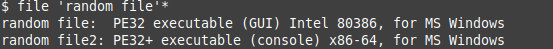
\includegraphics[width=\linewidth]{file_analysis.png}
	\caption{Output from using 'file' in Linux on 'random\_file' and 'random\_file1'}
	\label{fig:fileAnalysis}
\end{figure}

\subsubsection{Results} The 'PE32' and 'PE32+' indicate the file format is 'Portable Executable' (the '+' indicating version for 64bit memory structure)\cite{PE32Wikipedia}. The PE32 standard includes some headers in the file so the Windows operating can execute the files, either as a stand alone .exe files or as part of other programs or things running on the OS as .dll etc.\footnote{Windows file extensions for PE's include: .acm, .ax, .cpl, .dll, .drv, .efi, .exe, .mui, .ocx, .scr, .sys, .tsp, .mun\cite{PE32Wikipedia}} \\
I.e. the files could contain many functions for something running on a Windows OS. The PE file (ELF files for Linux) contain information of how the program should be laid out in memory on the OS.

\subsection{Reverse engineering, static analysis using Ghidra}
Static reverse engineering includes de-compiling the executables, looking at the code, but not running it. I used 'Ghidra'\cite{Ghidra } for the de-compilation. 




% \begin{figure}[!htp] % Single column figure
% 	\centering
% 	\includegraphics[width=\linewidth]{log1.png}
% 	\caption{Snippet from "log file 1.txt"}	\label{fig:log1}
% \end{figure}



%----------------------------------------------------------------------------------------
%	 REFERENCES
%----------------------------------------------------------------------------------------
\clearpage
\printbibliography % Output the bibliography

%----------------------------------------------------------------------------------------



%----------------------------------------------------------------------------------------
%	 Appendices
%----------------------------------------------------------------------------------------

\appendix


\clearpage
\chapter{Appendices}
\begin{appendices}
% \section{}\label{app:}	
% \begin{figure}[!htp] % Single column figure
% 	\centering
% 	\includegraphics[width=0.7\linewidth]{GPT1.png}
% 	\caption{ChatGPT analysis of logs before the large chunk of 'SERVER' logs}	\label{fig:GPT1.png}
% \end{figure}


\end{appendices}
\end{document}
